\documentclass[aspectratio=169, table]{beamer}


%\usepackage[beamertheme=./praditatheme]{Pradita}

\usetheme{Pradita}

\subtitle{IF231303-Software Architecture}
\title{\huge Chapter-10:\\Space-Based Architecture}
%\date[Serial]{\scriptsize {PRU/SPMI/FR-BM-18/0222}}
\author[Pradita]{\small {\textbf{David Eri, Khalid Husein, Ezra Christoper, Alfa Yohannis}}}


\begin{document}

    \frame{\titlepage}

    \begin{frame}
        \frametitle{Arsitektur Berbasis Ruang}
        \begin{itemize}
            \item Arsitektur Berbasis Ruang (SBA) adalah model komputasi terdistribusi untuk aplikasi berskala besar dan berkinerja tinggi.
            \item Ini menyediakan kerangka kerja yang dapat diskalakan untuk memproses dan mengelola data.
            \item SBA umumnya digunakan dalam analitik real-time, sistem perdagangan keuangan, dan platform permainan online.
        \end{itemize}
    \end{frame}

    \begin{frame}
        \frametitle{Sejarah}
        \begin{itemize}
            \item Arsitektur Berbasis Ruang memiliki akar sejarahnya pada tahun 1990-an ketika muncul sebagai respons terhadap kebutuhan akan sistem yang dapat diskalakan dan tahan terhadap kesalahan.
            \item Ini terinspirasi dari konsep-konsep seperti \textit{tuple spaces} (ruang-ruang pada memori dapat dipakai bersama) dan shared memory terdistribusi.
        \end{itemize}
    \end{frame}

    \begin{frame}{Arsitektur Berbasis Ruang}
        \vspace{30pt}
        \centering
        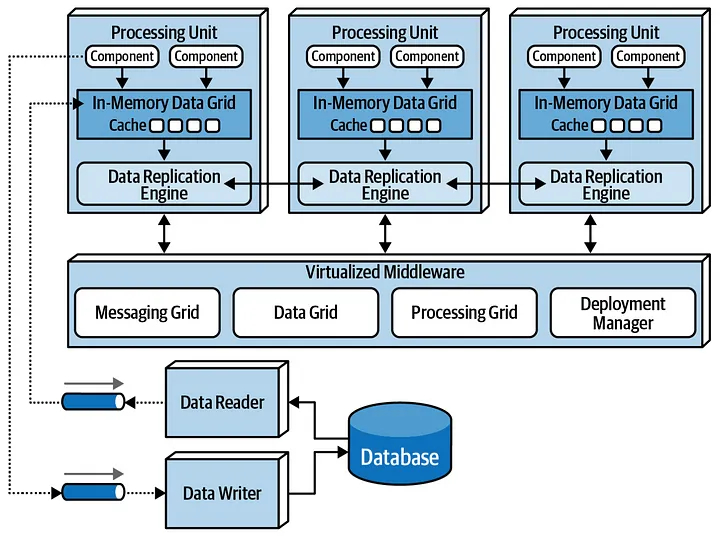
\includegraphics[width=0.7\textwidth]{../../images/spaced-based_architecture}
    \end{frame}

    \begin{frame}
        \frametitle{Komponen (1)}
        \begin{itemize}
            \item \textbf{Unit Pemrosesan}: Menjalankan logika aplikasi atau komputasi pada node terdistribusi.
            \item \textbf{In-Memory Data Grid}: Menyimpan data di memori untuk akses dan pemrosesan yang cepat.
            \item \textbf{Mesin Replikasi Data}: Memastikan kesamaan data dengan mereplikasi data di seluruh node.
            \item \textbf{Penulis Data}: Menulis data yang diterima unit pemrosesan ke Database.
            \item \textbf{Pembaca Data}: Membaca data dari Database ke In-Memory Data Grid.
            \item \textbf{Basis Data}: Penyimpanan data yang persisten (tahan lama).
        \end{itemize}
    \end{frame}

    \begin{frame}
        \frametitle{Komponen (2)}
        \vspace{20pt}
        \begin{itemize}
            \item \textbf{Middleware Virtual}: Mengabstraksi komunikasi antara komponen untuk integrasi yang mulus.
            \item \textbf{Grid Pesan}: Mengelola sesi dan permintaan dari pengguna dan mengalokasi tugas komputasi ke unit pemrosesan serta mengembalikan hasilnya.
            \item \textbf{Grid Data}: Mengelola sinkronisasi data antara data grid yang ada di masing-masing unit pemrosesan.
            \item \textbf{Grid Pemrosesan}: Mengkoordinasi tugas komputasi yang membutuhkan unit pemrosesan lebih dari satu, misalnya komputasi parallel.
            \item \textbf{Manajer Penempatan}: Mengatur penempatan dan penskalaan komponen. Misal dengan mengaktifkan dan menonaktifkan unit pemrosesan.
        \end{itemize}
    \end{frame}

    \begin{frame}
        \frametitle{Contoh}
        \begin{itemize}
            \item \textbf{Sistem Perdagangan Frekuensi Tinggi}: Institusi keuangan menggunakan SBA untuk memproses volume perdagangan besar secara real-time, memastikan latensi rendah dan throughput tinggi.
            \item \textbf{Platform Permainan Online}: Pengembang game memanfaatkan SBA untuk menangani lingkungan multipemain massal, memungkinkan permainan yang mulus dan pengiriman konten dinamis.
            \item \textbf{Jaringan Telekomunikasi}: Perusahaan telekomunikasi menggunakan SBA untuk mengelola lalu lintas jaringan, memastikan layanan komunikasi yang handal untuk jutaan pengguna.
        \end{itemize}
    \end{frame}

    \begin{frame}
        \frametitle{Kelebihan}
        \begin{itemize}
            \item \textbf{Skalabilitas}: SBA dapat diskalakan secara horizontal untuk menangani beban kerja yang semakin besar dengan menambahkan lebih banyak node.
            \item \textbf{Latensi Rendah}: Data disimpan di memori, menghasilkan operasi baca dan tulis yang cepat.
            \item \textbf{Throughput Tinggi}: SBA dapat memproses sejumlah besar transaksi secara bersamaan.
            \item \textbf{Query-intensive}: Cocok untuk sistem yang menangani permintaan baca (\textit{read requests}) yang banyak.
        \end{itemize}
    \end{frame}

    \begin{frame}
        \frametitle{Kekurangan}
        \begin{itemize}
            \item \textbf{Kompleksitas}: Implementasi dan pengelolaan sistem SBA dapat kompleks, membutuhkan keahlian dalam sistem terdistribusi.
            \item \textbf{Konsistensi}: Memastikan konsistensi data di seluruh node terdistribusi dapat menantang. Tidak cocok untuk sistem yang membutuhkan sikronisasi yang sering.
            \item \textbf{Konsumsi Sumber Daya}: Penyimpanan data di memori dapat mengkonsumsi jumlah sumber daya memori yang signifikan.
            \item \textbf{Variabilitas Latensi}: Latensi jaringan dan komunikasi node dapat memperkenalkan variabilitas dalam waktu tanggapan.
        \end{itemize}
    \end{frame}

    \begin{frame}
        \frametitle{Kesimpulan}
        \begin{itemize}
            \item Arsitektur Berbasis Ruang menawarkan kerangka kerja yang kuat untuk membangun sistem terdistribusi yang dapat diskalakan dan tahan terhadap kesalahan.
            \item Meskipun memberikan keuntungan signifikan seperti skalabilitas dan latensi rendah, ia juga datang dengan tantangan seperti kompleksitas dan pengelolaan konsistensi.
            \item Secara keseluruhan, SBA cocok untuk aplikasi yang membutuhkan kinerja tinggi, analitik real-time, dan toleransi terhadap kesalahan.
        \end{itemize}
    \end{frame}

\end{document}